% Credit Card Fraud Detection -- Architecture, Experiment Design & System Design
% Compile: tectonic architecture.tex  (figures are read from ../reports/figures/)
\documentclass[11pt,a4paper]{article}
\usepackage[a4paper,margin=22mm]{geometry}
\usepackage{fontspec}  % Unicode text so the copy-paste block copies real characters
\usepackage{hyperref}
\usepackage{amsmath,amssymb}
\usepackage{tikz}
\usetikzlibrary{shapes,arrows,positioning,calc,fit,backgrounds}
\usepackage{pgfplots}
\pgfplotsset{compat=1.18}
\usepackage{booktabs}
\usepackage{makecell}
\usepackage{array}
\newcolumntype{P}[1]{>{\raggedright\arraybackslash}p{#1}}
\usepackage{enumitem}
\usepackage{xcolor}
\usepackage{graphicx}
\graphicspath{{../reports/figures/}}
\usepackage{listings}
\hypersetup{colorlinks=true,linkcolor=blue!60!black,urlcolor=blue!60!black}
\setlength{\parskip}{4pt}
\setlength{\emergencystretch}{2.5em}
\tolerance=2000
\lstset{basicstyle=\ttfamily\scriptsize,frame=single,rulecolor=\color{black!30},
  backgroundcolor=\color{black!3},columns=fullflexible,keepspaces=true,
  showstringspaces=false,breaklines=true}
\tikzset{
flowbox/.style={rectangle,rounded corners,draw=black,thick,fill=black!4,
  text width=6.2cm,minimum height=1.05cm,align=center,font=\small},
flowstore/.style={ellipse,draw=black,thick,fill=black!8,align=center,font=\small},
flowarr/.style={thick,->,>=stealth},
badbox/.style={rectangle,rounded corners,draw=red!70!black,thick,fill=red!5,
  text width=6.4cm,minimum height=0.8cm,align=center,font=\footnotesize},
goodbox/.style={rectangle,rounded corners,draw=teal!70!black,thick,fill=teal!5,
  text width=6.4cm,minimum height=0.8cm,align=center,font=\footnotesize},
diagbox/.style={rectangle,rounded corners,draw=blue!70!black,thick,fill=blue!5,
  text width=5.2cm,minimum height=0.8cm,align=center,font=\footnotesize},
diagsmall/.style={rectangle,rounded corners,draw=black!70,thick,fill=black!4,
  text width=4.4cm,minimum height=0.75cm,align=center,font=\scriptsize}
}
% ---- champion retrain (filled from the audit run) ----
\newcommand{\retrainResult}{retrained from scratch (169\,s): identical metrics and threshold; scores within $2.2\times10^{-16}$ of the saved vector}

\title{Credit Card Fraud Detection\\{\large Architecture, Experiment Design \& System Design}}
\author{Project: \href{https://github.com/Divy18s/credit-card-fraud-detection}{\texttt{github.com/Divy18s/credit-card-fraud-detection}}\\
\small Classical ML $\cdot$ Gradient Boosting $\cdot$ Deep Learning $\cdot$ GAN oversampling $\cdot$ GNNs $\cdot$ SHAP}
\date{September 2026}
\begin{document}
\maketitle
\tableofcontents
\newpage

% ============================================================
\section{What was built}
Card fraud is rare, expensive to miss, and changes over time. The Kaggle ULB dataset used here has
284,807 card transactions over 48 hours with only \textbf{492 frauds (0.173\%)}. Its features are 28
anonymised PCA components (\texttt{V1}--\texttt{V28}) plus \texttt{Time} and \texttt{Amount}. There
are no cardholder, merchant or device IDs.

The project is a comparative study rather than a single model: \textbf{72 training runs} over
classical ML, gradient boosting, deep learning, GAN oversampling, ensembles and graph neural networks,
all under \emph{one} evaluation protocol designed to mirror deployment. It ships with:
\begin{itemize}[leftmargin=1.0cm]
\item \textbf{A chronological train / validation / test split} (70/15/15 by time): models learn from the
past and are scored on the future, exactly as a deployed model would be.
\item \textbf{Honest model selection:} resampling, class weights, hyperparameters, early stopping and
decision thresholds are all chosen on validation; the test window is scored once.
\item \textbf{Uncertainty, not just rankings:} a stratified bootstrap shows which differences are real.
\item \textbf{Explainability and a demo:} SHAP explanations of the champion, served in a Streamlit app.
\item \textbf{Ablations and a pre-registered replication} of a published benchmark.
\end{itemize}

{\footnotesize
\begin{center}
\begin{tabular}{@{}lP{4.6cm}P{7.2cm}@{}}
\toprule
Concern & Common approach & This project \\
\midrule
Split & random stratified shuffle & chronological 70/15/15 (train on past, test on future) \\
Resampling & SMOTE applied to the whole dataset before splitting & inside an \texttt{imblearn} pipeline: fitted on training rows only \\
Threshold & 0.5, or tuned on test & max-F1 threshold chosen on validation, frozen before test \\
Metric & accuracy / ROC-AUC & PR-AUC (average precision) first; F1, MCC, FP/FN counts \\
Class weight & $w=$ imbalance ratio (518) & selected on validation from a grid (ratio collapses LightGBM) \\
Comparison & single leaderboard & 1,000$\times$ stratified bootstrap CIs; paired tests \\
Model scope & one family & 18 model types, 8 imbalance strategies, GAN, stacking, GNNs, Optuna \\
Trust & results as reported & ablations, a pre-registration, documented errata, SHAP \\
\bottomrule
\end{tabular}
\end{center}
}

% ============================================================
\section{Technology stack}
{\footnotesize
\begin{center}
\begin{tabular}{@{}lP{4.6cm}P{7.2cm}@{}}
\toprule
Layer & Technology & Role \\
\midrule
Language & Python 3.12 & Everything \\
Data & pandas, NumPy & Loading, feature engineering, chronological splitting \\
Classical ML & scikit-learn 1.9 & Logistic regression, Random Forest, Decision Tree, Naive Bayes, calibrated LinearSVC \\
Boosting & XGBoost 3.4 (CUDA), LightGBM 4.7, CatBoost 1.2 (GPU) & Gradient-boosted trees with validation-selected \texttt{scale\_pos\_weight} \\
Imbalance & imbalanced-learn 0.14 & SMOTE, SMOTE-ENN, random undersampling inside \texttt{imblearn.Pipeline} \\
Deep learning & PyTorch 2.13 (CUDA 13, RTX 5050) & MLP, deep MLP, AutoEncoder, LSTM/BiLSTM, FT-Transformer, tabular GAN \\
Graphs & PyTorch Geometric 2.8 & GraphSAGE, GATv2 on $k$-NN transaction graphs \\
Tuning & Optuna (TPE, seed 42) & RF / XGBoost / LightGBM / CatBoost / GraphSAGE search on validation PR-AUC \\
Explainability & SHAP 0.52 (TreeExplainer) & Global and per-transaction attributions for the champion \\
App & Streamlit & Single-transaction scoring + SHAP waterfall, batch CSV scoring, leaderboard \\
Reporting & Jupyter, matplotlib, \LaTeX & EDA and final notebooks, report PDFs, this document \\
\bottomrule
\end{tabular}
\end{center}
}

% ============================================================
\section{System architecture}
\subsection{End-to-end pipeline}
\begin{center}
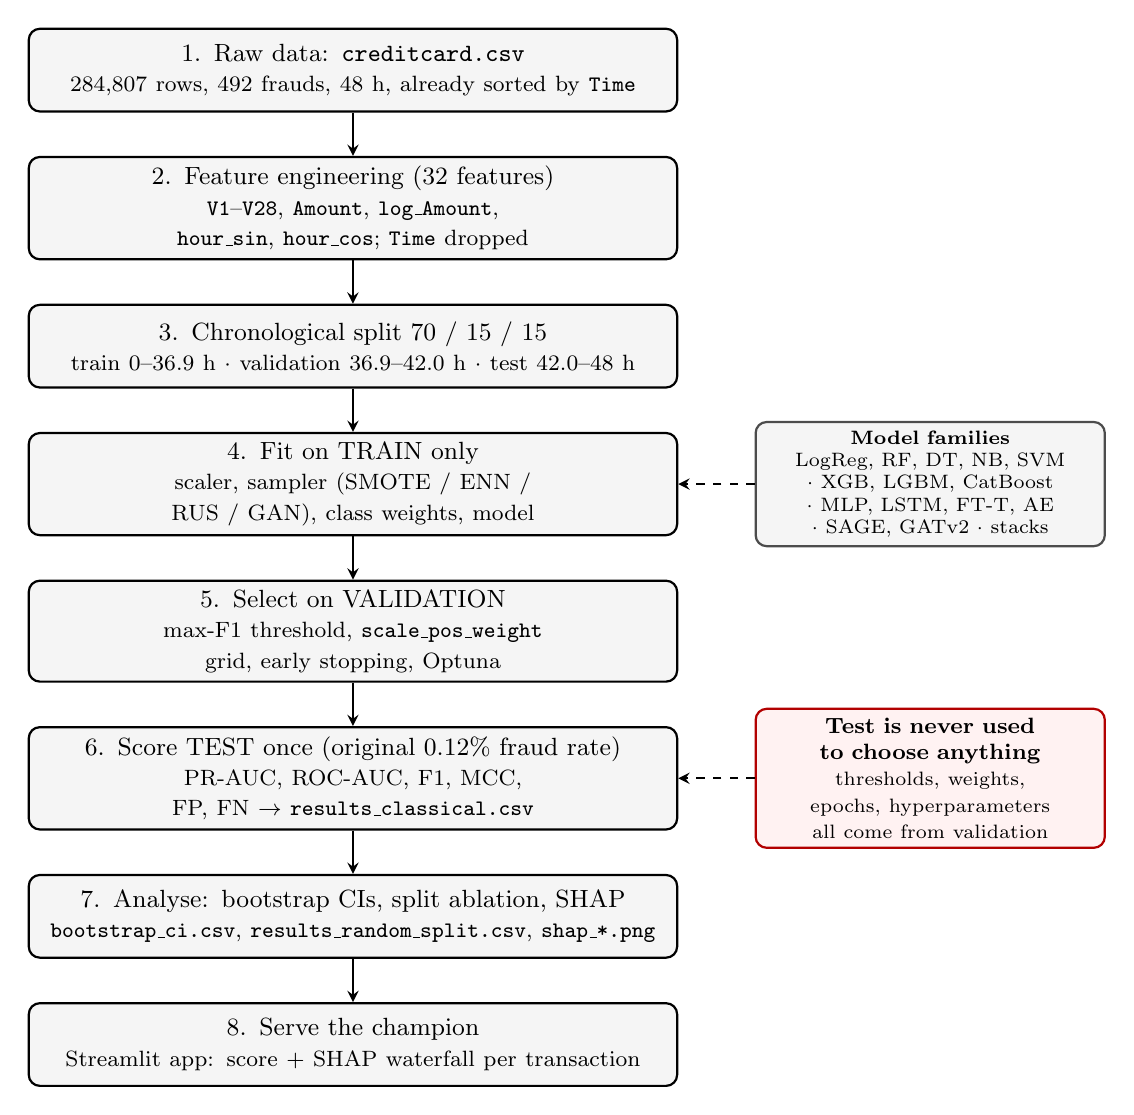
\begin{tikzpicture}[node distance=0.55cm,auto]
\tikzset{lc/.style={flowbox,text width=8.0cm}}
\node[lc] (raw) {1. Raw data: \texttt{creditcard.csv}\\\footnotesize 284,807 rows, 492 frauds, 48 h, already sorted by \texttt{Time}};
\node[lc,below=of raw] (feat) {2. Feature engineering (32 features)\\\footnotesize \texttt{V1}--\texttt{V28}, \texttt{Amount}, \texttt{log\_Amount}, \texttt{hour\_sin}, \texttt{hour\_cos}; \texttt{Time} dropped};
\node[lc,below=of feat] (split) {3. Chronological split 70 / 15 / 15\\\footnotesize train 0--36.9 h $\cdot$ validation 36.9--42.0 h $\cdot$ test 42.0--48 h};
\node[lc,below=of split] (fit) {4. Fit on TRAIN only\\\footnotesize scaler, sampler (SMOTE / ENN / RUS / GAN), class weights, model};
\node[lc,below=of fit] (sel) {5. Select on VALIDATION\\\footnotesize max-F1 threshold, \texttt{scale\_pos\_weight} grid, early stopping, Optuna};
\node[lc,below=of sel] (test) {6. Score TEST once (original 0.12\% fraud rate)\\\footnotesize PR-AUC, ROC-AUC, F1, MCC, FP, FN $\rightarrow$ \texttt{results\_classical.csv}};
\node[lc,below=of test] (post) {7. Analyse: bootstrap CIs, split ablation, SHAP\\\footnotesize \texttt{bootstrap\_ci.csv}, \texttt{results\_random\_split.csv}, \texttt{shap\_*.png}};
\node[lc,below=of post] (app) {8. Serve the champion\\\footnotesize Streamlit app: score + SHAP waterfall per transaction};
\coordinate (side) at ($(fit.east)+(3.2cm,0)$);
\node[diagsmall,text width=4.2cm] (fam) at (side |- fit) {\textbf{Model families}\\LogReg, RF, DT, NB, SVM $\cdot$ XGB, LGBM, CatBoost $\cdot$ MLP, LSTM, FT-T, AE $\cdot$ SAGE, GATv2 $\cdot$ stacks};
\node[badbox,text width=4.2cm] (never) at (side |- test) {\textbf{Test is never used to choose anything}\\\scriptsize thresholds, weights, epochs, hyperparameters all come from validation};
\foreach \a/\b in {raw/feat,feat/split,split/fit,fit/sel,sel/test,test/post,post/app} \draw[flowarr] (\a) -- (\b);
\draw[flowarr,dashed] (fam) -- (fit);
\draw[flowarr,dashed] (never) -- (test);
\end{tikzpicture}
\end{center}

\subsection{The chronological split and the drift it preserves}
\begin{center}
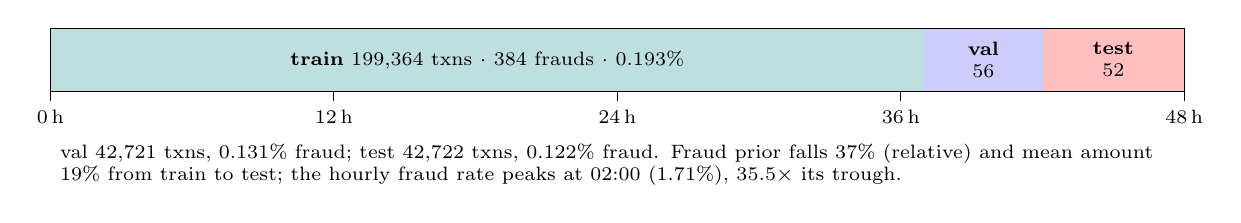
\begin{tikzpicture}[font=\scriptsize,>=stealth]
\def\sc{0.3}
\fill[teal!25] (0,0) rectangle (36.92*\sc,0.8);
\fill[blue!20] (36.92*\sc,0) rectangle (42.04*\sc,0.8);
\fill[red!25] (42.04*\sc,0) rectangle (48*\sc,0.8);
\draw (0,0) rectangle (48*\sc,0.8);
\node at (18.5*\sc,0.4) {\textbf{train} 199,364 txns $\cdot$ 384 frauds $\cdot$ 0.193\%};
\node[align=center] at (39.5*\sc,0.4) {\textbf{val}\\56};
\node[align=center] at (45*\sc,0.4) {\textbf{test}\\52};
\foreach \h in {0,12,24,36,48} {\draw (\h*\sc,0) -- (\h*\sc,-0.12) node[below]{\h\,h};}
\node[anchor=north west,align=left,text width=14.2cm] at (0,-0.55) {val 42,721 txns, 0.131\% fraud; test 42,722 txns, 0.122\% fraud.
Fraud prior falls 37\% (relative) and mean amount 19\% from train to test; the hourly fraud rate peaks at 02:00 (1.71\%), $35.5\times$ its trough.};
\end{tikzpicture}
\end{center}
Sorting by time and cutting at 70\% and 85\% means the model is always fitted on the past and scored on
the future. A random shuffle would erase this drift by making all three partitions look alike.

\subsection{Leakage-safe resampling: what happens at fit vs predict time}
\begin{center}
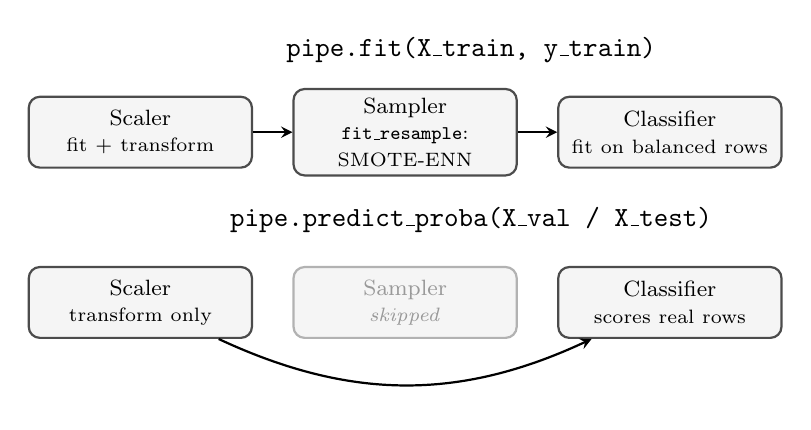
\begin{tikzpicture}[node distance=0.4cm and 0.5cm,auto,font=\footnotesize]
\tikzset{pb/.style={rectangle,rounded corners,draw=black!70,thick,fill=black!4,text width=2.6cm,align=center,minimum height=0.9cm}}
\node[font=\bfseries] (h1) at (0,0) {\texttt{pipe.fit(X\_train, y\_train)}};
\node[pb,below=0.3cm of h1,xshift=-4.2cm] (s1) {Scaler\\\scriptsize fit + transform};
\node[pb,right=of s1] (s2) {Sampler\\\scriptsize \texttt{fit\_resample}: SMOTE-ENN};
\node[pb,right=of s2] (s3) {Classifier\\\scriptsize fit on balanced rows};
\node[font=\bfseries] (h2) at ($(h1 |- s2.south)+(0,-0.55)$) {\texttt{pipe.predict\_proba(X\_val / X\_test)}};
\node[pb,below=0.3cm of h2,xshift=-4.2cm] (t1) {Scaler\\\scriptsize transform only};
\node[pb,right=of t1,draw=black!30,text=black!40] (t2) {Sampler\\\scriptsize \emph{skipped}};
\node[pb,right=of t2] (t3) {Classifier\\\scriptsize scores real rows};
\draw[flowarr] (s1) -- (s2); \draw[flowarr] (s2) -- (s3);
\draw[flowarr] (t1) to[bend right=25] (t3);
\end{tikzpicture}
\end{center}
\texttt{imblearn.Pipeline} applies samplers only during \texttt{fit}. Validation and test rows are never
resampled, so metrics are measured on the real 0.12\% fraud rate. Resampling \emph{before} splitting,
a common error in published work, would let synthetic copies of test frauds into training.

\subsection{Code layout}
{\footnotesize
\begin{center}
\begin{tabular}{@{}lP{10.0cm}@{}}
\toprule
File & Responsibility \\
\midrule
\texttt{src/config.py} & Paths, seed 42, split fractions \\
\texttt{src/data/dataset.py} & Load CSV, add features, chronological / random / Sang splits \\
\texttt{src/models/metrics.py} & Validation max-F1 threshold; PR-AUC, ROC-AUC, F1, MCC, confusion counts \\
\texttt{src/models/train\_classical.py} & 8 classical models $\times$ 7 imbalance strategies; \texttt{scale\_pos\_weight} grid on validation \\
\texttt{src/models/gan.py} & Tabular GAN for synthetic frauds; generator cached by a hash of the training frauds \\
\texttt{src/models/deep.py}, \texttt{train\_deep.py} & MLP, DNN, AutoEncoder, LSTM / BiLSTM (8-step windows), FT-Transformer; early stopping on validation \\
\texttt{src/models/gnn.py}, \texttt{train\_gnn.py} & $k$-NN graphs per split; GraphSAGE (full batch), GATv2 (sampled subgraphs) \\
\texttt{src/models/train\_ensembles.py} & 5-seed LSTM ensemble; RF + MLP + LSTM average \\
\texttt{src/models/tune\_optuna.py} & TPE search on validation PR-AUC \\
\texttt{src/models/ablation\_random\_split.py} & Same configs under chronological vs random split \\
\texttt{src/models/bootstrap\_ci.py} & Saves test score vectors; stratified bootstrap CIs \\
\texttt{src/models/explain\_shap.py} & Trains + saves the champion bundle; SHAP figures and summary \\
\texttt{app/streamlit\_app.py} & Demo app \\
\texttt{reports/} & Ledgers (CSV), score vectors (\texttt{.npz}), figures, report PDFs, pre-registration \\
\bottomrule
\end{tabular}
\end{center}
}

% ============================================================
\section{Step-by-step: technology, function, handling}
\subsection{Step 1 -- Features}
\textbf{Tech:} pandas, NumPy (\texttt{add\_features}).\\
\textbf{Does:} adds \texttt{log\_Amount} (tames the heavy-tailed amount) and a cyclical hour encoding
$(\sin\frac{2\pi h}{24}, \cos\frac{2\pi h}{24})$, so 23:00 and 00:00 are neighbours. \texttt{Time} itself
is dropped: a raw timestamp would let models memorise \emph{when} a window was, which can't generalise.\\
\textbf{Handles:} 32 model features in a fixed order, stored with the champion bundle so the app can't
feed columns in the wrong order.

\subsection{Step 2 -- Chronological split}
\textbf{Tech:} \texttt{time\_split}: sort by \texttt{Time}, cut at 70\% and 85\%.\\
\textbf{Does:} train on hours 0--36.9, choose on 36.9--42.0, test on 42.0--48.\\
\textbf{Handles:} exact duplicate rows share a \texttt{Time} value, so they stay together (0 cross the
boundary). The same module also builds the random split for the ablation, and Sang's 66/14/20 split,
which reproduces that paper's partition to the row (187,972 / 39,873 / 56,962; 368 / 49 / 75 frauds).

\subsection{Step 3 -- Imbalance strategies}
\textbf{Tech:} imbalanced-learn samplers inside \texttt{imblearn.Pipeline}; a PyTorch GAN.\\
\textbf{Does:} eight ways to handle 518:1 imbalance: do nothing; random undersampling to 1:1; SMOTE to
1:1; SMOTE followed by Edited Nearest Neighbours cleaning; class weights (validation-selected, or
fixed at the ratio); and GAN-generated frauds to 1:1.\\
\textbf{Handles:} samplers only ever see training rows (Section 3.3). For boosted trees,
\texttt{scale\_pos\_weight} is picked on validation from $\{1, 4, 16, \sqrt{r}, 64, r\}$, which prevents
the collapse that the textbook $w=r$ causes (LightGBM: PR-AUC 0.009 with 4,894 false positives).

\subsection{Step 4 -- Models}
\textbf{Tech:} scikit-learn, XGBoost/CatBoost on CUDA, LightGBM on CPU, PyTorch, PyTorch Geometric.\\
\textbf{Does:} 18 model types. Sequence models see the last 8 transactions as a window; graph models
see a 10-nearest-neighbour graph built separately inside each split; the FT-Transformer tokenises each
feature; the AutoEncoder learns legitimate traffic only and flags high reconstruction error.\\
\textbf{Handles:} neural nets and GNNs early-stop on validation PR-AUC; seeds fixed at 42.

\subsection{Step 5 -- Threshold and metrics}
\textbf{Tech:} \texttt{best\_threshold\_f1} (validation), \texttt{evaluate\_scores} (test).\\
\textbf{Does:} the threshold maximising F1 on validation is frozen, then test is scored once.\\
\textbf{Handles:} thresholds in the ledger range from 0.07 to 1.0; a fixed 0.5 would be badly wrong for
most models. PR-AUC is the headline because its baseline equals the fraud rate (0.0012 on test),
whereas ROC-AUC looks excellent ($>0.95$) even for mediocre fraud detectors.

\subsection{Step 6 -- Bootstrap, ablation, SHAP, app}
\textbf{Tech:} saved score vectors (\texttt{.npz}); stratified bootstrap; TreeExplainer; Streamlit.\\
\textbf{Does:} turns single numbers into intervals; measures what the split protocol is worth; explains
the champion; serves it.\\
\textbf{Handles:} the app samples only from the held-out test window (rows 242,085--284,806, verified
identical to the training code's test split) and loads a bundle of \{pipeline, threshold, feature order\}.

% ============================================================
\section{Deep-dive: handling 0.17\% fraud}
\subsection{The techniques}
\begin{itemize}[leftmargin=1.0cm]
\item \textbf{SMOTE} creates synthetic frauds on the line between a fraud $x_i$ and one of its $k=5$
nearest fraud neighbours $x_{nn}$: \quad $x_{\text{new}} = x_i + \lambda\,(x_{nn} - x_i),\ \lambda \sim U(0,1)$.
\item \textbf{ENN} then deletes any row whose class disagrees with the majority of its 3 nearest
neighbours, cleaning the noisy boundary SMOTE tends to create.
\item \textbf{Class weighting} multiplies the loss on frauds by $w$ (\texttt{scale\_pos\_weight},
\texttt{pos\_weight}); no rows are added.
\item \textbf{GAN}: a generator maps noise $z\sim\mathcal{N}(0,I_{24})$ to synthetic fraud rows while a
discriminator learns to tell them from real frauds (label smoothing 0.9, 8,000 steps). The cache key
is a SHA-1 of the training frauds, so a generator trained on one split is never reused on another.
\end{itemize}

\subsection{Results grid (test PR-AUC, best per strategy in bold)}
{\footnotesize
\begin{center}
\begin{tabular}{@{}lccccc@{}}
\toprule
Strategy & LogReg & Random Forest & XGBoost & LightGBM & CatBoost \\
\midrule
raw & 0.649 & 0.749 & 0.714 & 0.537 & \textbf{0.752} \\
random undersampling & 0.627 & \textbf{0.768} & 0.723 & 0.756 & 0.670 \\
SMOTE & 0.729 & \textbf{0.790} & 0.770 & 0.770 & 0.743 \\
SMOTE-ENN & 0.738 & \textbf{0.795} & 0.777 & 0.768 & 0.755 \\
class weight (val-selected) & 0.720 & \textbf{0.784} & 0.769 & 0.537 & 0.765 \\
GAN & 0.568 & 0.762 & 0.769 & 0.775 & \textbf{0.783} \\
\bottomrule
\end{tabular}
\end{center}
}
Hybrid SMOTE-ENN gives the champion (RF, 0.795). GAN synthesis is best for CatBoost and rescues LightGBM,
but hurts the linear model; for sequences, weighting beats both SMOTE-ENN (0.758) and GAN (0.750)
because interpolating time windows distorts their dynamics. Validation-selected weights are the fix
for the collapse above: Optuna independently chose moderate weights too (4--172, never 518).

% ============================================================
\section{Deep-dive: why a chronological split}
\subsection{The validity argument}
A random split trains on transactions that happen \emph{after} the ones it is scored on. No deployed
system can do that, so the number answers a question with no operational counterpart. That argument
holds even if both protocols scored the same. Two measurable channels follow from shuffling:
\begin{enumerate}[leftmargin=1.0cm]
\item \textbf{Temporal ordering destroyed:} late fraud patterns inform early predictions, and the drift
of Section 3.2 disappears.
\item \textbf{Duplicates separated:} ULB has 1,081 extra copies of rows in 773 groups. Shuffling puts
517 of them across partition boundaries (249 train$\to$test, 207 train$\to$val, 61 val$\to$test); the
chronological split puts 0. Duplicates are also informative: 14.3\% of \texteuro0.00 duplicates are
fraud (card testing), against a 0.173\% base rate.
\end{enumerate}
A third channel, resampling before splitting, is excluded by construction (Section 3.3), so every
effect measured here is a floor for what the protocol is worth in published work.

\subsection{Measured effect (same code, only the split assignment changes)}
{\footnotesize
\begin{center}
\begin{tabular}{@{}lccc@{}}
\toprule
Configuration & chronological & random & random $-$ chronological \\
\midrule
XGBoost + class weight & 0.7688 & 0.8372 & $+0.0684$ \\
CatBoost + GAN & 0.7804 & 0.8399 & $+0.0595$ \\
MLP raw & 0.7794 & 0.8267 & $+0.0473$ \\
XGBoost + SMOTE-ENN & 0.7766 & 0.8104 & $+0.0338$ \\
RF + SMOTE-ENN & 0.7947 & 0.8120 & $+0.0173$ \\
LSTM + class weight & 0.7803 & 0.7965 & $+0.0162$ \\
GraphSAGE + class weight & 0.7389 & 0.6948 & $-0.0441$ \\
\midrule
\multicolumn{3}{@{}l}{Pooled over 10 paired runs (7 at 70/15/15, 3 at 66/14/20)} & $\mathbf{+0.0182}$, 7/10 positive \\
\bottomrule
\end{tabular}
\end{center}
}
The pooled 95\% CI is $[-0.0084, +0.0448]$ ($t=1.55$; one-sided sign test $p = 176/1024 = 0.172$). The
project reports this honestly: the data establish the \emph{direction}, not a reliable magnitude.
GraphSAGE is the exception: shuffling scrambles the temporal coherence of its neighbourhoods.

\subsection{Pre-registered replication of a published split}
Sang (2026) reports XGBoost PR-AUC 0.7902 on a 66/14/20 chronological split of the same CSV. The
question, the three configurations and the reading were written down and committed before running:
{\footnotesize
\begin{center}
\begin{tabular}{@{}lcccc@{}}
\toprule
Configuration & 70/15/15 & 66/14/20 & $\Delta$ split & vs 0.7902 \\
\midrule
XGBoost + class weight & 0.7688 & \textbf{0.8055} & $+0.0367$ & $+0.0153$ (0.37 SE) \\
XGBoost + SMOTE-ENN & 0.7766 & 0.8102 & $+0.0336$ & $+0.0200$ (0.48 SE) \\
RF + SMOTE-ENN & 0.7947 & 0.8224 & $+0.0276$ & $+0.0322$ (0.77 SE) \\
\bottomrule
\end{tabular}
\end{center}
}
Read as a replication, not an improvement: the closest analogue lands 0.37 SE from the published value
(SE $\approx 0.050\sqrt{52/75} \approx 0.042$) and recovers the same 57 of 75 frauds. The bigger finding is
that the cut point alone moved PR-AUC by $+0.033$ on average, more than the pooled protocol effect.

% ============================================================
\section{Deep-dive: how much can 52 test frauds tell us?}
\subsection{PR-AUC and the bootstrap}
Average precision summarises the precision--recall curve over ranked scores:
\begin{equation}
\text{AP} = \sum_n (R_n - R_{n-1})\,P_n, \qquad \text{baseline (random scores)} = \frac{\#\text{frauds}}{\#\text{rows}} = \frac{52}{42{,}722} \approx 0.0012
\end{equation}
To get an interval, the test set is resampled 1,000 times \emph{stratified}: the 52 frauds and the
42,670 legitimate rows are each resampled with replacement, so every replicate keeps the real class
balance. The 2.5th and 97.5th percentiles of AP form the 95\% CI.

\begin{center}
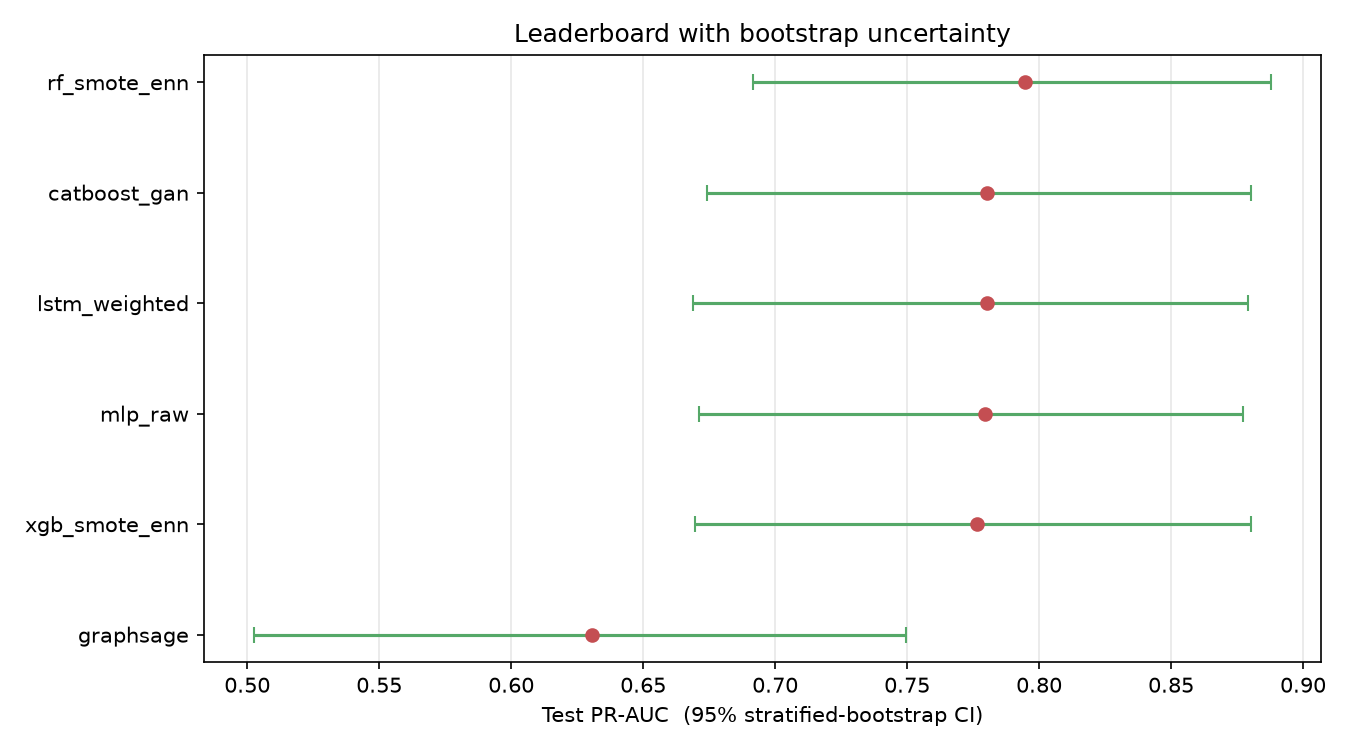
\includegraphics[width=0.78\textwidth]{bootstrap_ci.png}
\end{center}
{\footnotesize
\begin{center}
\begin{tabular}{@{}lccc@{}}
\toprule
Representative config & PR-AUC & 95\% CI & width \\
\midrule
RF + SMOTE-ENN & 0.7947 & [0.692, 0.888] & 0.196 \\
CatBoost + GAN & 0.7804 & [0.674, 0.880] & 0.206 \\
LSTM + class weight & 0.7803 & [0.669, 0.879] & 0.210 \\
MLP raw & 0.7794 & [0.671, 0.877] & 0.206 \\
XGBoost + SMOTE-ENN & 0.7766 & [0.670, 0.880] & 0.211 \\
GraphSAGE + class weight & 0.7242 & [0.601, 0.837] & 0.236 \\
\bottomrule
\end{tabular}
\end{center}
}
\textbf{All 15 pairwise intervals overlap.} A paired bootstrap of RF vs XGBoost (same resamples for both)
gives a difference of $+0.018$ with a CI that includes zero. And one transaction is worth about
$\pm0.020$: promoting the worst-ranked test fraud to the top moves PR-AUC by $+0.0198$, demoting the
best-ranked to the bottom by $-0.0199$. The honest output is a shared band of roughly 0.72--0.89,
\emph{not} a ranking.

% ============================================================
\section{Results}
\subsection{Best configuration of each model type (test window, 52 frauds)}
{\footnotesize
\begin{center}
\begin{tabular}{@{}llccccc@{}}
\toprule
Model & Strategy & PR-AUC & ROC-AUC & F1 & MCC & FP / FN \\
\midrule
\textbf{Random Forest} & \textbf{SMOTE-ENN} & \textbf{0.7947} & 0.971 & \textbf{0.848} & \textbf{0.855} & 1 / 13 \\
RF + MLP + LSTM & stacked average & 0.7850 & 0.984 & 0.835 & 0.844 & 1 / 14 \\
CatBoost & GAN & 0.7825 & 0.972 & 0.848 & 0.855 & 1 / 13 \\
BiLSTM & class weight & 0.7811 & 0.980 & 0.839 & 0.844 & 2 / 13 \\
LSTM & class weight & 0.7799 & 0.971 & 0.813 & 0.821 & 2 / 15 \\
XGBoost & SMOTE-ENN & 0.7766 & 0.973 & 0.812 & 0.815 & 5 / 13 \\
LightGBM & GAN & 0.7752 & 0.981 & 0.822 & 0.832 & 1 / 15 \\
MLP & raw & 0.7746 & 0.971 & 0.809 & 0.821 & 1 / 16 \\
GraphSAGE & class weight & 0.7558 & 0.923 & 0.796 & 0.801 & 4 / 15 \\
GATv2 & class weight & 0.7448 & 0.966 & 0.783 & 0.789 & 4 / 16 \\
Logistic regression & SMOTE-ENN & 0.7379 & 0.975 & 0.767 & 0.785 & 1 / 19 \\
FT-Transformer & class weight & 0.6811 & 0.980 & 0.760 & 0.760 & 10 / 14 \\
AutoEncoder & anomaly score & 0.5845 & 0.941 & 0.660 & 0.660 & 19 / 17 \\
Decision Tree & class weight & 0.4054 & 0.855 & 0.632 & 0.636 & 28 / 15 \\
\bottomrule
\end{tabular}
\end{center}
}

\begin{center}
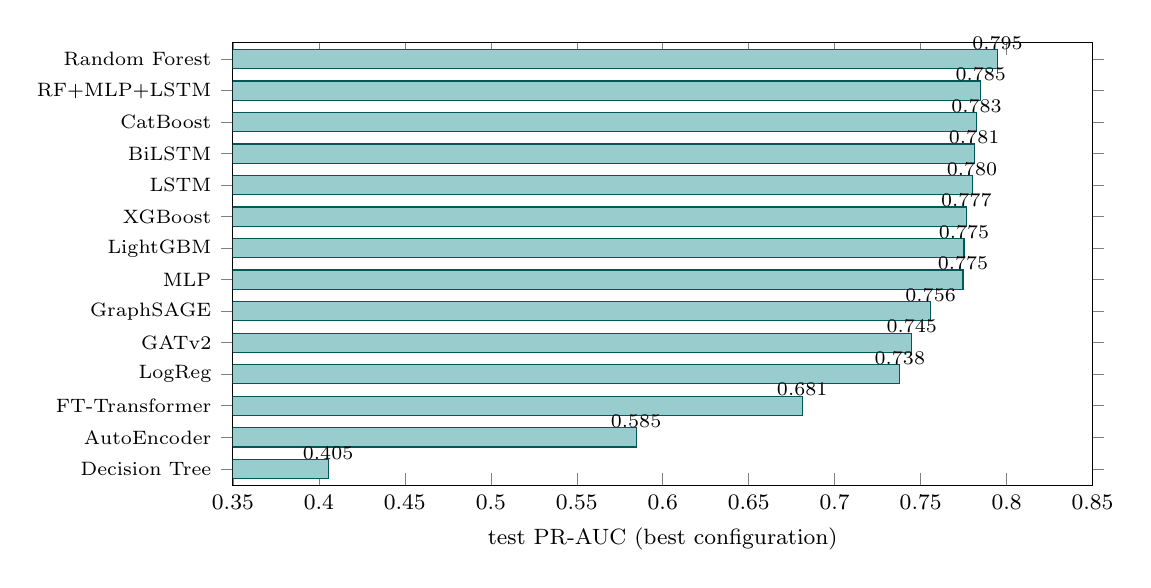
\begin{tikzpicture}
\begin{axis}[xbar,width=12.5cm,height=7.2cm,bar width=7pt,xmin=0.35,xmax=0.85,
  symbolic y coords={Decision Tree,AutoEncoder,FT-Transformer,LogReg,GATv2,GraphSAGE,MLP,LightGBM,XGBoost,LSTM,BiLSTM,CatBoost,RF+MLP+LSTM,Random Forest},
  ytick=data,y tick label style={font=\scriptsize},xlabel={test PR-AUC (best configuration)},
  nodes near coords,nodes near coords style={font=\scriptsize},point meta=explicit symbolic,
  font=\footnotesize,enlarge y limits=0.04]
\addplot[fill=teal!40,draw=teal!70!black] coordinates {
  (0.4054,Decision Tree) [0.405] (0.5845,AutoEncoder) [0.585] (0.6811,FT-Transformer) [0.681]
  (0.7379,LogReg) [0.738] (0.7448,GATv2) [0.745] (0.7558,GraphSAGE) [0.756] (0.7746,MLP) [0.775]
  (0.7752,LightGBM) [0.775] (0.7766,XGBoost) [0.777] (0.7799,LSTM) [0.780] (0.7811,BiLSTM) [0.781]
  (0.7825,CatBoost) [0.783] (0.7850,RF+MLP+LSTM) [0.785] (0.7947,Random Forest) [0.795]};
\end{axis}
\end{tikzpicture}
\end{center}

\subsection{What the grid says}
\begin{itemize}[leftmargin=1.0cm]
\item \textbf{Ensembles of trees win; a single tree fails.} RF 0.795 vs its own Decision Tree 0.405.
\item \textbf{Diversity beats seeds.} RF + MLP + LSTM (0.785) beats every deep model; a 5-seed LSTM
ensemble (0.775) doesn't beat its own best member.
\item \textbf{Depth and attention don't help on 32 PCA features.} A 512-256-128-64 DNN ties the small MLP
(0.7752 vs 0.7746); the FT-Transformer trails both.
\item \textbf{Graphs without entities $\approx$ an MLP.} A feature-similarity graph carries signal (SAGE
0.756) but no real relational structure; published graph results ($\approx$0.89) need cardholder and
merchant IDs, which this dataset doesn't have.
\item \textbf{Tuning repairs, it doesn't lift.} Optuna took LightGBM from 0.537 to 0.753 and XGBoost raw
from 0.714 to 0.769, but every family's best stays within $\pm0.01$.
\item \textbf{Unsupervised isn't enough.} The AutoEncoder reaches ROC-AUC 0.94 but PR-AUC only 0.58.
\end{itemize}

\subsection{Champion operating point}
At its validation-chosen threshold (0.718) the champion flags 40 of 42,722 test transactions: \textbf{39
frauds and 1 legitimate}, missing 13. That is 97.5\% precision at 75\% recall. In an operations
setting, nearly every alert an analyst opens is real.

% ============================================================
\section{Explainability (SHAP)}
\begin{center}
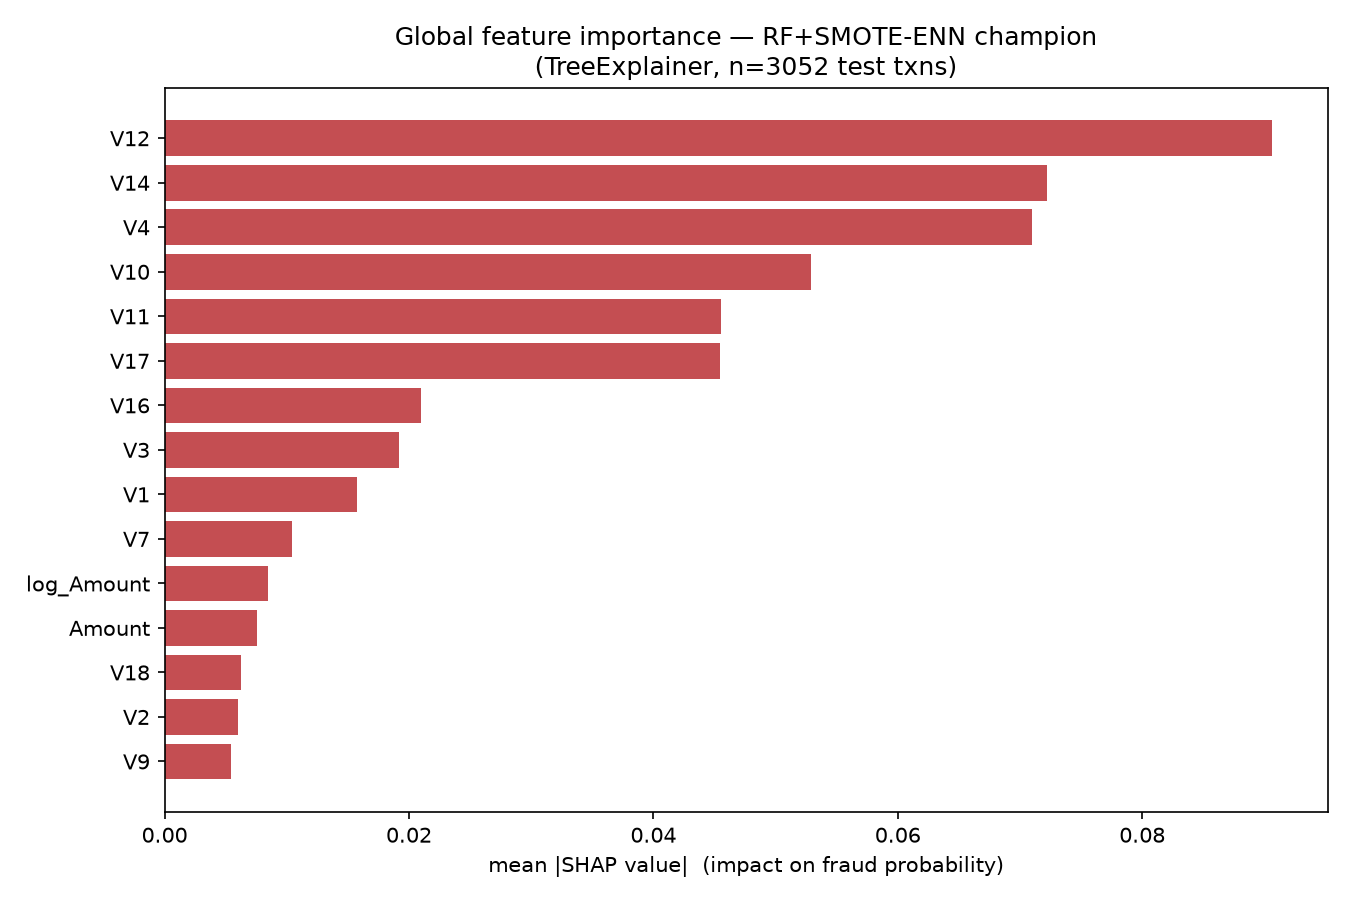
\includegraphics[width=0.72\textwidth]{shap_global_importance.png}
\end{center}
TreeExplainer on 3,052 test rows (all 52 frauds + 3,000 random legitimate). Top drivers: \texttt{V12},
\texttt{V14}, \texttt{V4}, \texttt{V10}, \texttt{V11}, \texttt{V17}. Low \texttt{V12/V14/V10/V17} and high
\texttt{V4/V11} push toward fraud, matching the signs of the EDA correlations. Shapley values
decompose each prediction additively, $f(x) = \phi_0 + \sum_j \phi_j$, which is what the app's per-transaction
waterfall shows.

% ============================================================
\section{Audit: what was checked, and what was found}
\subsection{Recomputed from the raw data and saved artifacts}
{\footnotesize
\begin{center}
\begin{tabular}{@{}P{6.0cm}P{6.2cm}c@{}}
\toprule
Claim & Recomputed & Status \\
\midrule
Dataset: 284,807 rows, 492 frauds, 0.173\% & 284,807 / 492 / 0.173\% & \checkmark \\
Split sizes, frauds, hours, fraud rates, mean amounts & all 15 values identical & \checkmark \\
Prior $-37\%$, amount $-19\%$, peak 02:00 at 1.71\%, $35.5\times$ & $-36.8\%$, $-19.2\%$, 02:00 / 1.71\%, $35.5\times$ & \checkmark \\
1,081 duplicates in 773 groups; 517 leak randomly, 0 chronologically & 1,081 / 773; 249 + 207 + 61 = 517; 0 & \checkmark \\
Card-testing rates 14.3\% (\texteuro0) and 4.6\% (\texteuro0.01--2) & 14.3\% and 4.6\% & \checkmark \\
Sang splits reproduce exactly; shuffled test has 98 frauds & 187,972 / 39,873 / 56,962; 368 / 49 / 75; 98 & \checkmark \\
Champion: PR-AUC 0.795, F1 0.848, MCC 0.855, 1 FP, 13 FN & saved model re-scored: 0.7947, 0.8478, 0.8550, 1, 13 & \checkmark \\
Champion reproduces from code & \retrainResult & \checkmark \\
Bootstrap CIs (6 configs) and ``all 15 pairs overlap'' & all 6 CIs identical to 4 d.p.; 15 / 15 overlap & \checkmark \\
One transaction $\approx\pm0.020$ PR-AUC & $+0.0198$ / $-0.0199$; single-fraud removal range 0.0203 & \checkmark \\
XGBoost + class weight: 0.7688 chronological / 0.8372 random & re-run: 0.7688 (spw 16, 2 FP / 16 FN) / 0.8372 & \checkmark \\
Pooled $+0.0182$, 7/10 positive, sign test $p=0.172$ & recomputed from the three ledgers & \checkmark \\
Tuned results (LGBM 0.753, XGB 0.769, RF 0.782, CatBoost 0.766) & present in the ledger & \checkmark \\
Pre-registration committed before the replication run & 04:04:41 pre-registration, 04:16:29 result (backup branch) & \checkmark \\
Demo app loads, scores, explains & served headless; single-transaction and leaderboard tabs render & \checkmark \\
\bottomrule
\end{tabular}
\end{center}
}

\subsection{Issues found (none changes a headline result)}
\begin{enumerate}[leftmargin=1.0cm]
\item \textbf{GATv2 early stopping uses the training graph.} \texttt{train\_gat\_minibatch} computes its
``validation'' AP on the same graph it trains on; the docstring says validation. Measured in a scratch
re-run: shipped code 0.7684 test PR-AUC (1-hop inference) / 0.7698 (exact 2-hop inference); corrected
(early stopping on the validation graph) 0.7329; ledger 0.7448. GATv2 lands at 0.73--0.77 every way,
so ``attention adds cost, not accuracy'' stands, but the row is one draw from a spread of 0.037 (0.733--0.770).
\item \textbf{GAT inference comment is inaccurate.} \texttt{predict\_minibatch} says ``no edges are lost'',
but a 2-layer model gets only 1-hop context. The effect is tiny (0.7684 vs 0.7698).
\item \textbf{Graph models see future features within a window.} Each split's $k$-NN graph links a
transaction to later transactions in the same window (features only, never labels). A deployed
system couldn't see those. It affects GraphSAGE and GATv2 only.
\item \textbf{Duplicate leakage is understated.} The 517 counts byte-identical rows including
\texttt{Time}, which isn't a model input. Rows identical in the 32 features the models actually see:
\textbf{1,784} under the random split vs 8 chronologically (0 train$\to$test, none of them frauds). This
strengthens the project's argument.
\item \textbf{Paired RF vs XGBoost test isn't in the code.} README: $+0.0187$, CI $[-0.0119, +0.0515]$.
Recomputed from the saved scores: point $+0.0181$ (bootstrap mean $+0.0188$), CI $[-0.0116, +0.0510]$.
Same conclusion; the script should be committed and the point estimate quoted.
\item \textbf{Two results aren't in any file.} The XGBoost + class weight random-split run (0.8372) and
the Optuna parameters of the four boosters (\texttt{optuna\_best\_params.json} holds only GraphSAGE).
The first was reproduced exactly by re-running; the second can't be traced.
\item \textbf{The public history can't show the pre-registration.} \texttt{main} on GitHub was squashed
into one commit; the ordering evidence exists only on the local branch \texttt{backup-main-history}.
\item \textbf{Maintenance.} Streamlit's \texttt{use\_container\_width} is deprecated (warned for removal
after 2025-12-31); \texttt{ablation\_random\_split.run\_gnn} hard-codes \texttt{"cuda"}, so it fails on a
CPU-only machine.
\end{enumerate}

% ============================================================
\section{System design decisions (interview-ready)}
\begin{enumerate}[leftmargin=1.2cm]
\item \textbf{Evaluate the way you deploy.} Train on the past, test on the future; select on a window in
between. Any other protocol answers a question production never asks.
\item \textbf{Put every data-dependent step inside the pipeline.} Scalers and samplers are fitted with the
model on training rows only, so resampling can't leak.
\item \textbf{Test is read once.} Thresholds, class weights, epochs and hyperparameters come from
validation. The one ``fixed-weight'' variant is kept as a documented failure, not tuned away.
\item \textbf{Rank with PR-AUC, report with counts.} At 0.12\% prevalence ROC-AUC flatters everything;
PR-AUC plus FP/FN counts is what an operations team can use.
\item \textbf{Intervals before rankings.} With 52 test frauds, one transaction is worth $\pm0.02$; claims
smaller than that are noise.
\item \textbf{Fingerprint cached artifacts.} The GAN cache is keyed by a hash of the training frauds after
an early run reused one generator across protocols (documented as an erratum).
\item \textbf{Ship the model with its contract.} The joblib bundle holds pipeline, threshold and feature
order together.
\end{enumerate}

\subsection{Likely interview questions}
{\footnotesize
\begin{center}
\begin{tabular}{@{}P{4.6cm}P{11.2cm}@{}}
\toprule
Question & Answer \\
\midrule
Why not accuracy or ROC-AUC? & Predicting ``legit'' for everything is 99.88\% accurate. ROC-AUC counts true negatives, which are
abundant, so even weak models score above 0.95. PR-AUC's baseline is the prevalence (0.0012), so it
measures what matters: how clean the top of the ranking is. \\
Why SMOTE inside the pipeline? & If you oversample first and split later, synthetic neighbours of test frauds end up in training:
the model is graded on near-copies of what it learned. \\
Why did $w = 518$ break LightGBM? & Huge weights make every leaf split chase the positives; the model predicted fraud on 4,894
legitimate test rows. Selecting $w$ on validation (it chose 1) avoids it. \\
Is RF really the best? & It has the highest point estimate, but its CI overlaps every other tier's; the paired test
against XGBoost includes zero. The defensible claim is a band, not a winner. \\
Why is the random split higher? & Shuffling mixes future patterns into training and separates duplicates across the boundary; it
also erases drift. The pooled gain is $+0.018$ with a CI including zero, so the magnitude is uncertain,
but the protocol is invalid regardless. \\
How would this change in production? & Add real entities (card, merchant, device) for velocity features and genuine graphs; retrain on
a rolling window; calibrate scores; monitor precision at the alert threshold as fraud drifts; and
account for label delay (chargebacks arrive weeks later). \\
\bottomrule
\end{tabular}
\end{center}
}

% ============================================================
\section{Limitations and future work}
\begin{itemize}[leftmargin=1.0cm]
\item \textbf{48 hours, 52 test frauds.} Every comparison is statistically loose; a longer dataset is
the real fix.
\item \textbf{Anonymised PCA features, no entity IDs.} Rules out velocity features and true relational
graphs.
\item \textbf{Single chronological cut.} Rolling-origin (walk-forward) evaluation would show how stable
the ranking is over time.
\item \textbf{Run-to-run variance} for neural and graph models (0.01--0.04) is larger than
several leaderboard gaps; multi-seed means would be more robust.
\item \textbf{No cost model.} Threshold selection maximises F1; a production system would weigh the
cost of a missed fraud against the cost of an analyst review.
\end{itemize}

% ============================================================
\section{Resume entry}
\begingroup\small
\noindent{\footnotesize\textbf{Credit Card Fraud Detection} $|$ {\scriptsize\emph{Python, scikit-learn, XGBoost, PyTorch, PyTorch Geometric}} \textbf{\color{blue!60!black}\href{https://github.com/Divy18s/credit-card-fraud-detection}{(GITHUB)}} \hfill\mbox{Aug 2026}}
\begin{itemize}[leftmargin=0.8cm,itemsep=2pt]
\item Benchmarked \textbf{72 fraud-detection pipelines} across classical ML, gradient boosting, LSTM/Transformer, GAN oversampling and GNNs on \textbf{284,807 transactions (0.17\% fraud)} under a chronological split with in-pipeline resampling and validation-only tuning.
\item Delivered a \textbf{Random Forest + SMOTE-ENN} champion with \textbf{PR-AUC 0.795 and F1 0.848}, reaching \textbf{97.5\% precision at 75\% recall with 1 false positive in 42,722} future transactions, served in a \textbf{Streamlit} app with per-prediction \textbf{SHAP} explanations.
\item Quantified uncertainty with a \textbf{1,000$\times$ stratified bootstrap}: 95\% CIs span \textbf{0.20--0.24} and \textbf{all 15 model pairs overlap}, with one test fraud worth \textbf{$\pm$0.020 PR-AUC}, so results are reported as a performance band rather than a false ranking.
\item Showed random shuffling leaks \textbf{517 duplicate rows} across partitions (0 chronologically) and \textbf{pre-registered a replication} of a published benchmark, landing \textbf{0.37 SE} from its PR-AUC (0.8055 vs 0.7902).
\end{itemize}
\endgroup

\subsection{Plain text for copy-paste}
Select the box and copy. No hyphenation or ligatures, so words paste intact; the same text is in
\texttt{docs/resume\_entry.txt}.

\medskip
\noindent\fcolorbox{black!30}{black!3}{\begin{minipage}{\dimexpr\linewidth-2\fboxsep-2\fboxrule\relax}
% Straight quotes, no fi/fl ligatures, no hyphenation: copies back exactly as typed.
\small\fontspec{lmroman10-regular.otf}[Ligatures={NoCommon,TeXOff}]\raggedright\hyphenpenalty=10000\exhyphenpenalty=10000
\setlength{\parskip}{7pt}\setlength{\parindent}{0pt}
Credit Card Fraud Detection | Python, scikit-learn, XGBoost, PyTorch, PyTorch Geometric (GITHUB) — Aug 2026

• Benchmarked 72 fraud-detection pipelines across classical ML, gradient boosting, LSTM/Transformer, GAN oversampling and GNNs on 284,807 transactions (0.17\% fraud) under a chronological split with in-pipeline resampling and validation-only tuning.

• Delivered a Random Forest + SMOTE-ENN champion with PR-AUC 0.795 and F1 0.848, reaching 97.5\% precision at 75\% recall with 1 false positive in 42,722 future transactions, served in a Streamlit app with per-prediction SHAP explanations.

• Quantified uncertainty with a 1,000× stratified bootstrap: 95\% CIs span 0.20–0.24 and all 15 model pairs overlap, with one test fraud worth ±0.020 PR-AUC, so results are reported as a performance band rather than a false ranking.

• Showed random shuffling leaks 517 duplicate rows across partitions (0 chronologically) and pre-registered a replication of a published benchmark, landing 0.37 SE from its PR-AUC (0.8055 vs 0.7902).
\end{minipage}}

\section{Thirty-second pitch}
``I compared 72 fraud-detection pipelines, from logistic regression to LSTMs, GANs and graph neural
networks, on 284,807 card transactions where only 0.17\% are fraud. The key decision was the protocol:
train on the past and test on the future, with resampling and thresholds chosen only on validation,
because that's how a deployed model is used. The best model, a Random Forest with SMOTE-ENN, catches
three quarters of frauds at 97.5\% precision, one false alarm in 42,722 transactions, and every prediction
is explained with SHAP in a Streamlit app. But I also bootstrapped the test set and found all the top
models' intervals overlap, so the honest result is a performance band, not a winner.''

\appendix
\section{Reproduce}
\begin{lstlisting}
python -m venv .venv && .venv\Scripts\activate && pip install -r requirements.txt
python -m src.data.make_dataset                     # download creditcard.csv (Kaggle token)
python -m src.models.train_classical                # classical + boosting grid
python -m src.models.train_deep                     # MLP / LSTM / FT-Transformer / AutoEncoder
python -m src.models.train_gnn                      # GraphSAGE / GATv2
python -m src.models.train_ensembles                # LSTM ensemble, RF+MLP+LSTM stack
python -m src.models.tune_optuna                    # Optuna tuning
python -m src.models.ablation_random_split          # chronological vs random
python -m src.models.train_classical --split sang   # pre-registered replication
python -m src.models.bootstrap_ci                   # CIs from saved score vectors
python -m src.models.explain_shap                   # champion bundle + SHAP figures
.venv\Scripts\streamlit run app/streamlit_app.py    # demo
\end{lstlisting}
\end{document}
